% \iffalse
\let\negmedspace\undefined
\let\negthickspace\undefined
\documentclass[journal,12pt,twocolumn]{IEEEtran}
\usepackage{cite}
\usepackage{amsmath,amssymb,amsfonts,amsthm}
\usepackage{algorithmic}
\usepackage{graphicx}
\usepackage{textcomp}
\usepackage{xcolor}
\usepackage{txfonts}
\usepackage{listings}
\usepackage{enumitem}
\usepackage{mathtools}
\usepackage{gensymb}
\usepackage{comment}
\usepackage[breaklinks=true]{hyperref}
\usepackage{tkz-euclide} 
\usepackage{listings}
\usepackage{gvv}                                        
\def\inputGnumericTable{}                                 
\usepackage[latin1]{inputenc}                                
\usepackage{color}                                            
\usepackage{array}                                            
\usepackage{longtable}                              
\usepackage{calc}                                             
\usepackage{multirow}                                         
\usepackage{hhline}                                           
\usepackage{ifthen}                                           
\usepackage{lscape}

\newtheorem{theorem}{Theorem}[section]
\newtheorem{problem}{Problem}
\newtheorem{proposition}{Proposition}[section]
\newtheorem{lemma}{Lemma}[section]
\newtheorem{corollary}[theorem]{Corollary}
\newtheorem{example}{Example}[section]
\newtheorem{definition}[problem]{Definition}
\newcommand{\BEQA}{\begin{eqnarray}}
\newcommand{\EEQA}{\end{eqnarray}}
\newcommand{\define}{\stackrel{\triangle}{=}}
\theoremstyle{remark}
\newtheorem{rem}{Remark}
\begin{document}

\bibliographystyle{IEEEtran}
\vspace{3cm}

\title{NCERT DISCRETE}
\author{EE23BTECH11020 - Raghava Ganji$^{*}$% <-this % stops a space
}
\maketitle
\newpage
\bigskip

\renewcommand{\thefigure}{\theenumi}
\renewcommand{\thetable}{\theenumi}

\textbf{GATE 2023 BM.48:}
The function $f(z)=\frac{1}{z-1}$ of a complex variable Z on a closed counter in an anti-clockwise direction.For which of the following counters, does this integral have a non-zero value?\\
\brak{A}$\abs{z-2}=0.01$\\
\brak{B}$\abs{z-1}=0.1$\\
\brak{C}$\abs{z-3}=5$\\
\brak{D}$\abs{z}=2$\\
\solution\\
For the integral to have a non-zero value, the contour must enclose the singularity of the function.\\\\
For $\oint_{c}f\brak zdz$ the singularity exists at $z=1$.\\\\
Above given all the contours are circles. Therefore which contour encloses $z=1$, then the given integral have a non-zero value.\\\\
\begin{figure}
    \centering
    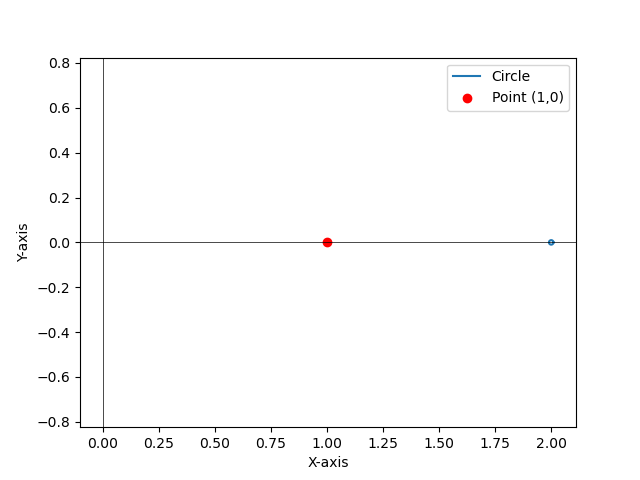
\includegraphics[width=1\columnwidth]{plotg231.png}
    \caption{graph of option A}
\end{figure}
\begin{figure}
    \centering
    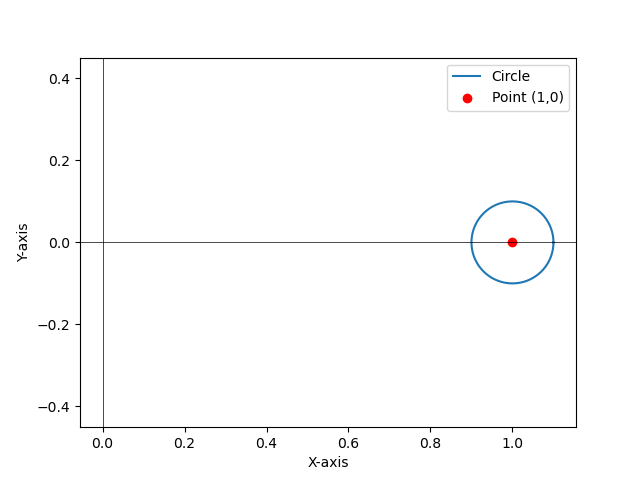
\includegraphics[width=1\columnwidth]{plotg232.png}
    \caption{graph of option B}
\end{figure}
\begin{figure}
    \centering
    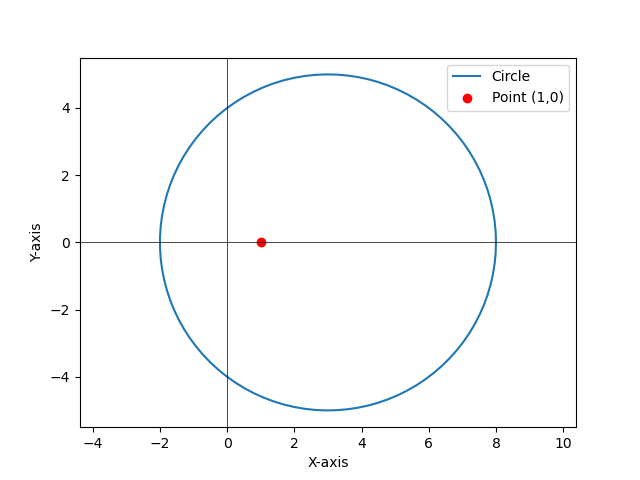
\includegraphics[width=1\columnwidth]{plotg233.png}
    \caption{graph of option C}
\end{figure}
\begin{figure}
    \centering
    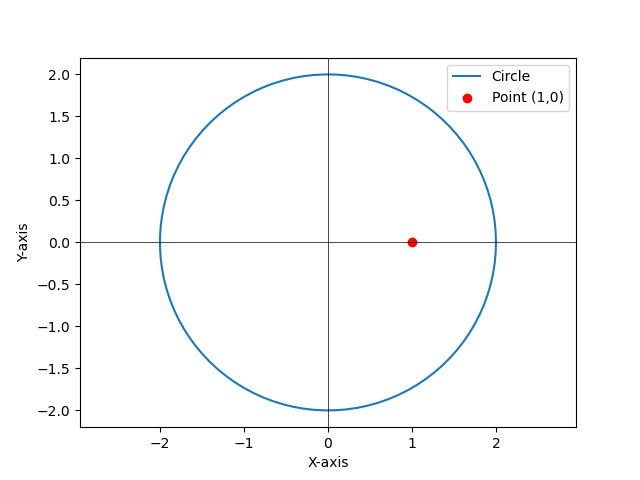
\includegraphics[width=1\columnwidth]{plotg234.png}
    \caption{graph of option D}
\end{figure}
After analysing all the graphs that we understand for options B,C,D contours encloses $z=1$. 
\end{document}
